% Format teze zasnovan je na paketu memoir
% http://tug.ctan.org/macros/latex/contrib/memoir/memman.pdf ili
% http://texdoc.net/texmf-dist/doc/latex/memoir/memman.pdf
% 
% Prilikom zadavanja klase memoir, navedenim opcijama se podešava 
% veličina slova (12pt) i jednostrano štampanje (oneside).
% Ove parametre možete menjati samo ako pravite nezvanične verzije
% mastera za privatnu upotrebu (na primer, u b5 varijanti ima smisla 
% smanjiti 
\documentclass[11pt,oneside]{memoir}

% Paket koji definiše sve specifičnosti mastera Matematičkog fakulteta
\usepackage{matfmaster}
%
% Podrazumevano pismo je ćirilica.
%   Ako koristite pdflatex, a ne xetex, sav latinički tekst na srpskom jeziku
%   treba biti okružen sa \lat{...} ili \begin{latinica}...\end{latinica}.
%
% Opicija [latinica]:
%   ako želite da pišete latiniciom, dodajte opciju "latinica" tj.
%   prethodni paket uključite pomoću: \usepackage[latinica]{matfmaster}.
%   Ako koristite pdflatex, a ne xetex, sav ćirilički tekst treba biti
%   okružen sa \cir{...} ili \begin{cirilica}...\end{cirilica}.
%
% Opcija [biblatex]:
%   ako želite da koristite reference na više jezika i umesto paketa
%   bibtex da koristite BibLaTeX/Biber, dodajte opciju "biblatex" tj.
%   prethodni paket uključite pomoću: \usepackage[biblatex]{matfmaster}
%
% Opcija [b5paper]:
%   ako želite da napravite verziju teze u manjem (b5) formatu, navedite
%   opciju "b5paper", tj. prethodni paket uključite pomoću: 
%   \usepackage[b5paper]{matfmaster}. Tada ima smisla razmisliti o promeni
%   veličine slova (izmenom opcije 12pt na 11pt u \documentclass{memoir}).
%
% Naravno, opcije je moguće kombinovati.
% Npr. \usepackage[b5paper,biblatex]{matfmaster}

% Pomoćni paket koji generiše nasumičan tekst u kojem se javljaju sva slova
% azbuke (nema potrebe koristiti ovo u pravim disertacijama)
\usepackage{pangrami}

% Paket koji obezbeđuje ispravni prikaz ćiriličkih italik slova kada
% se koristi pdflatex. Zakomentarisati ako na sistemu koji koristite ovaj
% paket nije dostupan ili ako ne radi ispravno.
\usepackage{cmsrb}

% Ostali paketi koji se koriste u dokumentu
\usepackage{listings} % listing programskog koda
\usepackage{hyperref}

% Datoteka sa literaturom u BibTex tj. BibLaTeX/Biber formatu
\bibliography{matfmaster-primer}

% Ime kandidata na srpskom jeziku (u odabranom pismu)
\autor{Момир Аџемовић}
% Naslov teze na srpskom jeziku (u odabranom pismu)
\naslov{Предикциjа траjекториjа више обjеката на сцени}
% Godina u kojoj je teza predana komisiji
\godina{2022}
% Ime i afilijacija mentora (u odabranom pismu)
\mentor{др Младен Николић, ванредни професор\\ Универзитет у Београду, Математички факултет}
% Ime i afilijacija prvog člana komisije (u odabranom pismu)
\komisijaA{др Јована Ковачевић, доцент\\ Универзитет у Београду, Математички факултет}
% Ime i afilijacija drugog člana komisije (u odabranom pismu)
\komisijaB{др Александар Картељ, доцент\\ Универзитет у Београду, Математички факултет}
% Ime i afilijacija trećeg člana komisije (opciono)
% \komisijaC{}
% Ime i afilijacija četvrtog člana komisije (opciono)
% \komisijaD{}
% Datum odbrane (obrisati ili iskomentarisati narednu liniju ako datum odbrane nije poznat)
\datumodbrane{15. септембар 2022.}

% Apstrakt na srpskom jeziku (u odabranom pismu)
\apstr{%
У изради...
}

% Ključne reči na srpskom jeziku (u odabranom pismu)
\kljucnereci{машинско учење, аутономна вожња, графовске неуронске мреже}

\begin{document}
% ==============================================================================
% Uvodni deo teze
\frontmatter
% ==============================================================================
% Naslovna strana
\naslovna
% Strana sa podacima o mentoru i članovima komisije
\komisija
% Strana sa posvetom (u odabranom pismu)
\posveta{посвета... у изради...}
% Strana sa podacima o disertaciji na srpskom jeziku
\apstrakt
% Sadržaj teze
\tableofcontents*

% ==============================================================================
% Glavni deo teze
\mainmatter
% ==============================================================================

% ------------------------------------------------------------------------------
\chapter{Увод}
% ------------------------------------------------------------------------------

У изради...

% ------------------------------------------------------------------------------
\chapter{Припрема података}

Основни скуп података за тренирање и тестирање техника предикције трајекторија је \textit{Argoverse Motion Forecasting} скуп података
који се састоји од детаљних мапа саобраћаја (\textit{eng. ,,HD maps``}) које садрже геометријске и семантичке податке сцена. Постоје две \textit{HD} сцене
за градове Питсбург и у Мајами. Коришћењем аутономних возила су генерисани сценарији који представљају неколико узастопних слика сцена (у табеларном формату)
на деловима мапа. Сви детаљи о овом скупу података се могу пронаћи на адреси 
\href{https://www.argoverse.org/index.html}{\color{blue}{www.argoverse.org}} \cite{argoverse}. \\


\noindent Kључне информације које се издвајају из сваког сценарију су:
\begin{itemize}
  \item Мапа сценарија (Питсбург или Мајами);
  \item Трајекторије агената;
  \item Трајекторије осталих објеката на сцени;
  \item Возне (централне) линије.
\end{itemize}

\section{Претпроцесирање података}

\noindent Подаци сваког сценарија се векторизују и чувају у полу-структуираном формату. 
За парсирање и обраду улазних података се користи \textit{argoverse API} интерфејс.


Трајекторија агента\footnote{Низ $(x, y)$ тачака, где је приближна временска разлика између две тачке око 0.1 секунде} 
се дели на два дела: историја (својства) и реализација (будуће вредности). Реализација се састоји од $N_r$ 
опажања $x$ и $y$ релативних координата\footnote{Све координате се нормализују тако да су релативне у односу на последње опажање у трајекторији историје агента} 
тј. облик реализације је $(N_r, 2)$. 
Историја се аналогно формира да садржи историју $N_h$ опажања $x$ i $y$ релативних координата. Овај део трајекторије иде непосредно
пре реализације. Посматрамо следеће случајеве:
\begin{itemize}
  \item Постоји више од $N_h + N_r$ опажања: Одбацује се реп трајекторије (првих неколико вредности хронолошки гледано);
  \item Постоји мање од $N_{hmin} + N_r$ опажања: Сценарио се одбацује (сматра се да је невалидан);
  \item Постоји између $N_{hmin} + N_r$ и $N_h + N_r$ опажања: реп трајекторије се допуњава до димензије $N_h + N_r$ 
  посматрано као да објекат мирује у тим тренуцима.
\end{itemize}
Коначно, облик историје је $(N_h, 3)$, где трећа вредност означава да ли је опажање право ($1$) или допуњено ($0$).

Трајекторије суседних објеката се деле на два дела аналогно трајекторији агента. Неопходно је да се синхронизују трајекторије 
суседних објеката по временским ознакама (eng. \textit{timestamp}) са трајекторијом агента, јер не постоји у сваком тренутку исти
број објеката на сцени. Након синхронизације се трајекторије деле на историју и реализацију и проверава се да ли дужине тих
делова задовољавају критеријуме:
\begin{itemize}
  \item Уколико је дужина трајекторије историје краћа од $N_{homin}$, онда се објекат одбацује;
  \item Уколико је дужина трајекторије реализације краћа од $N_{romin}$, онда се објекат одбацује.
\end{itemize}
Као додатна провера, за сваки сусед се провера растојање од агента. Уколико је сусед превише далеко, онда се се он одбацује.
Критеријум за одбацивање суседа узима у обзир брзину агента (по $x$ и $y$ оси одвоједно) и растојање њихових последњих опажања
у трајекторији историје. Уколико неки од следећих услова није
испуњен, сусед се игнорише у сценарију: $\frac{O_n^x}{A_s^x} \leq T_{steps}$, $\frac{O_n^y}{A_s^y} \leq T_{steps}$,
где је $O_n^x$ ($O_n^y$) нормализована $x$ ($y$) координата суседа, $А_s^x$ ($А_s^y$) је наивно 
апроксимирана\footnote{Брзина се апроксимира као просек промена координата у трајекторији историје} брзина агента
по $x$ ($y$) оси и $T_{steps}$ је параметар толеранције.
Трајекторије се секу или допуњавају до фиксног облика. Векторизован облик: $(N_n, N_h, 3)$ и $(N_n, N_r, 3)$, где је $N_n$ број
судедних објеката. 

На основу локације агента се издвајају сегменти централних линија (возне путање) које нису даље од агента за више од $D_{lsinit}$. Уколико нема
пронађених сегмената централних линија, онда се вредност за $D_{lsinit}$ множи $K_{ls}$\footnote{$D_{lsinit}$ и $K_{ls}$ су фиксне вредности
у \textit{argoverse} интерфејсу} 
пута до највише $D_{lsmax}$ (ако и даље нема сегмената, 
онда се сценарио одбацује). За сваки сегмент се чува низ од 10 $(x, y)$ координата приширених са метаподацима:
\begin{itemize} 
  \item \texit{is\_intersection} - да ли се сегмент сече са неким сегментом,
  \item \textit{turn\_right} - да ли је у питању скретање у десно, 
  \item \textit{turn\_left} - да ли је у питању скретање у лево, 
  \item \textit{turn\_none} - да ли нема стретања, 
  \item \textit{is\_traffic\_control} - да ли постоји контрола саобраћаја. 
\end{itemize}
Коначан облик је $(N_{ls}, 10, 7)$. 

Скуп кандидата централних сегмената линија за предикције трајекторија: Постоји коначан број централних сегмената линија по којој
објекат може да се креће у скоријој будућности, због чега је корисно да се као улаз у модел користе централне линије као кандидати. 
Основа алгоритма за проналазак ових кандидата се налази у \textit{argoverse} интерфејсу \cite{argoverse}. Кандидати се проналазе
коришћењем трајекторије историје агента. Коначан векторизован облик је: $(N_c, N_r, 3)$, где је $N_c$ број пронађених кандидата,
$N_r$ дужина трајекторије реализације. Пошто се централне линије допуњавају по потреби до димензије $N_r$, користи се трећа координата
за маску. Погледати табелу \ref{dp-params-table} за преглед свих параметара процеса.

\begin{table}
  \begin{tabular}{C|C}
    Ознака параметра & Објашњење \\
    \hline
    $N_r$ & Дужина трајекторије реализације (део који се предвиђа) \\
    $N_h$ & Дужина трајекторија историје \\
    $N_{hmin}$ & Минимална дужина трајекторије историје пре допуњавања \\
    $N_{hоmin}$ & Минимална дужина трајекторије историје суседа пре допуњавања \\
    $N_{rоmin}$ & Минимална дужина трајекторије реализације суседа пре допуњавања \\
    $T_{steps}$ & Умножак максималног растојања до сегмента централне линије \\
    $D_{lsmax}$ & Максимално растојање до централне линије
  \end{tabular}
  \caption{Преглед параметара припреме података}
  \label{dp-params-table}
\end{table}

На сликама \ref{scenario-example-3700} и \ref{scenario-example-4791} се налазе примери два визуализована сценарија
након претходне припреме. У овом формату нису прикази делови сцене на којој је могућа вожња, али 
постоје (централне линије) тј. путање по којима се возила најчњшће крећу. Изузеци су у случају неких скретања,
промени линија, ...

\begin{figure}[h!]
  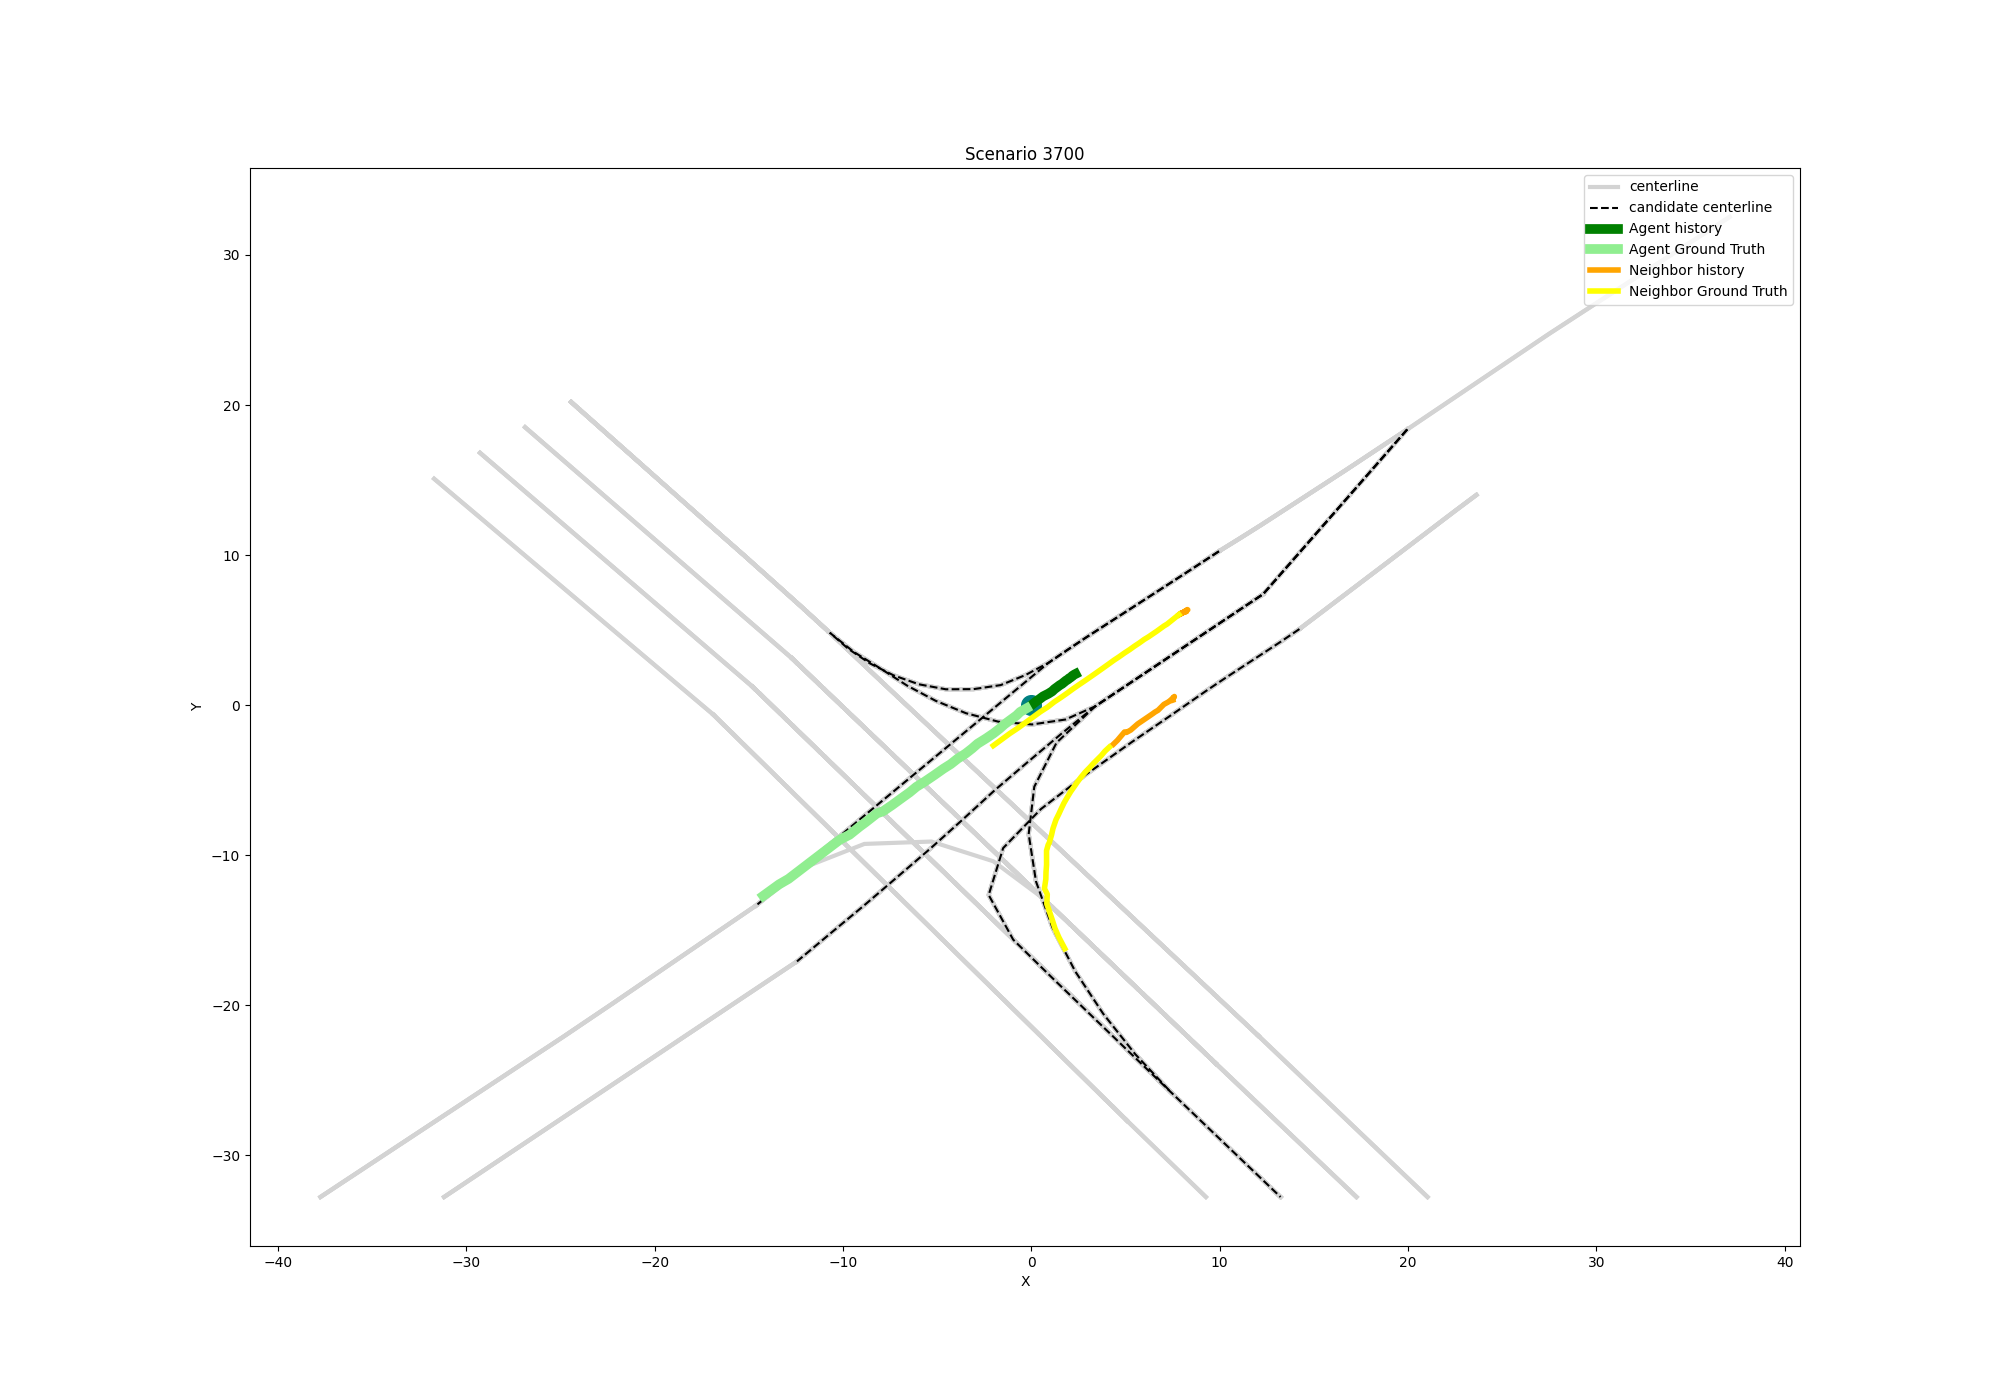
\includegraphics[width=0.9\textwidth]{images/scenario3700.png}
  \caption{Визуализација припремљених података - Пример 1}
  \label{scenario-example-3700}
\end{figure}

\begin{figure}[h!]
  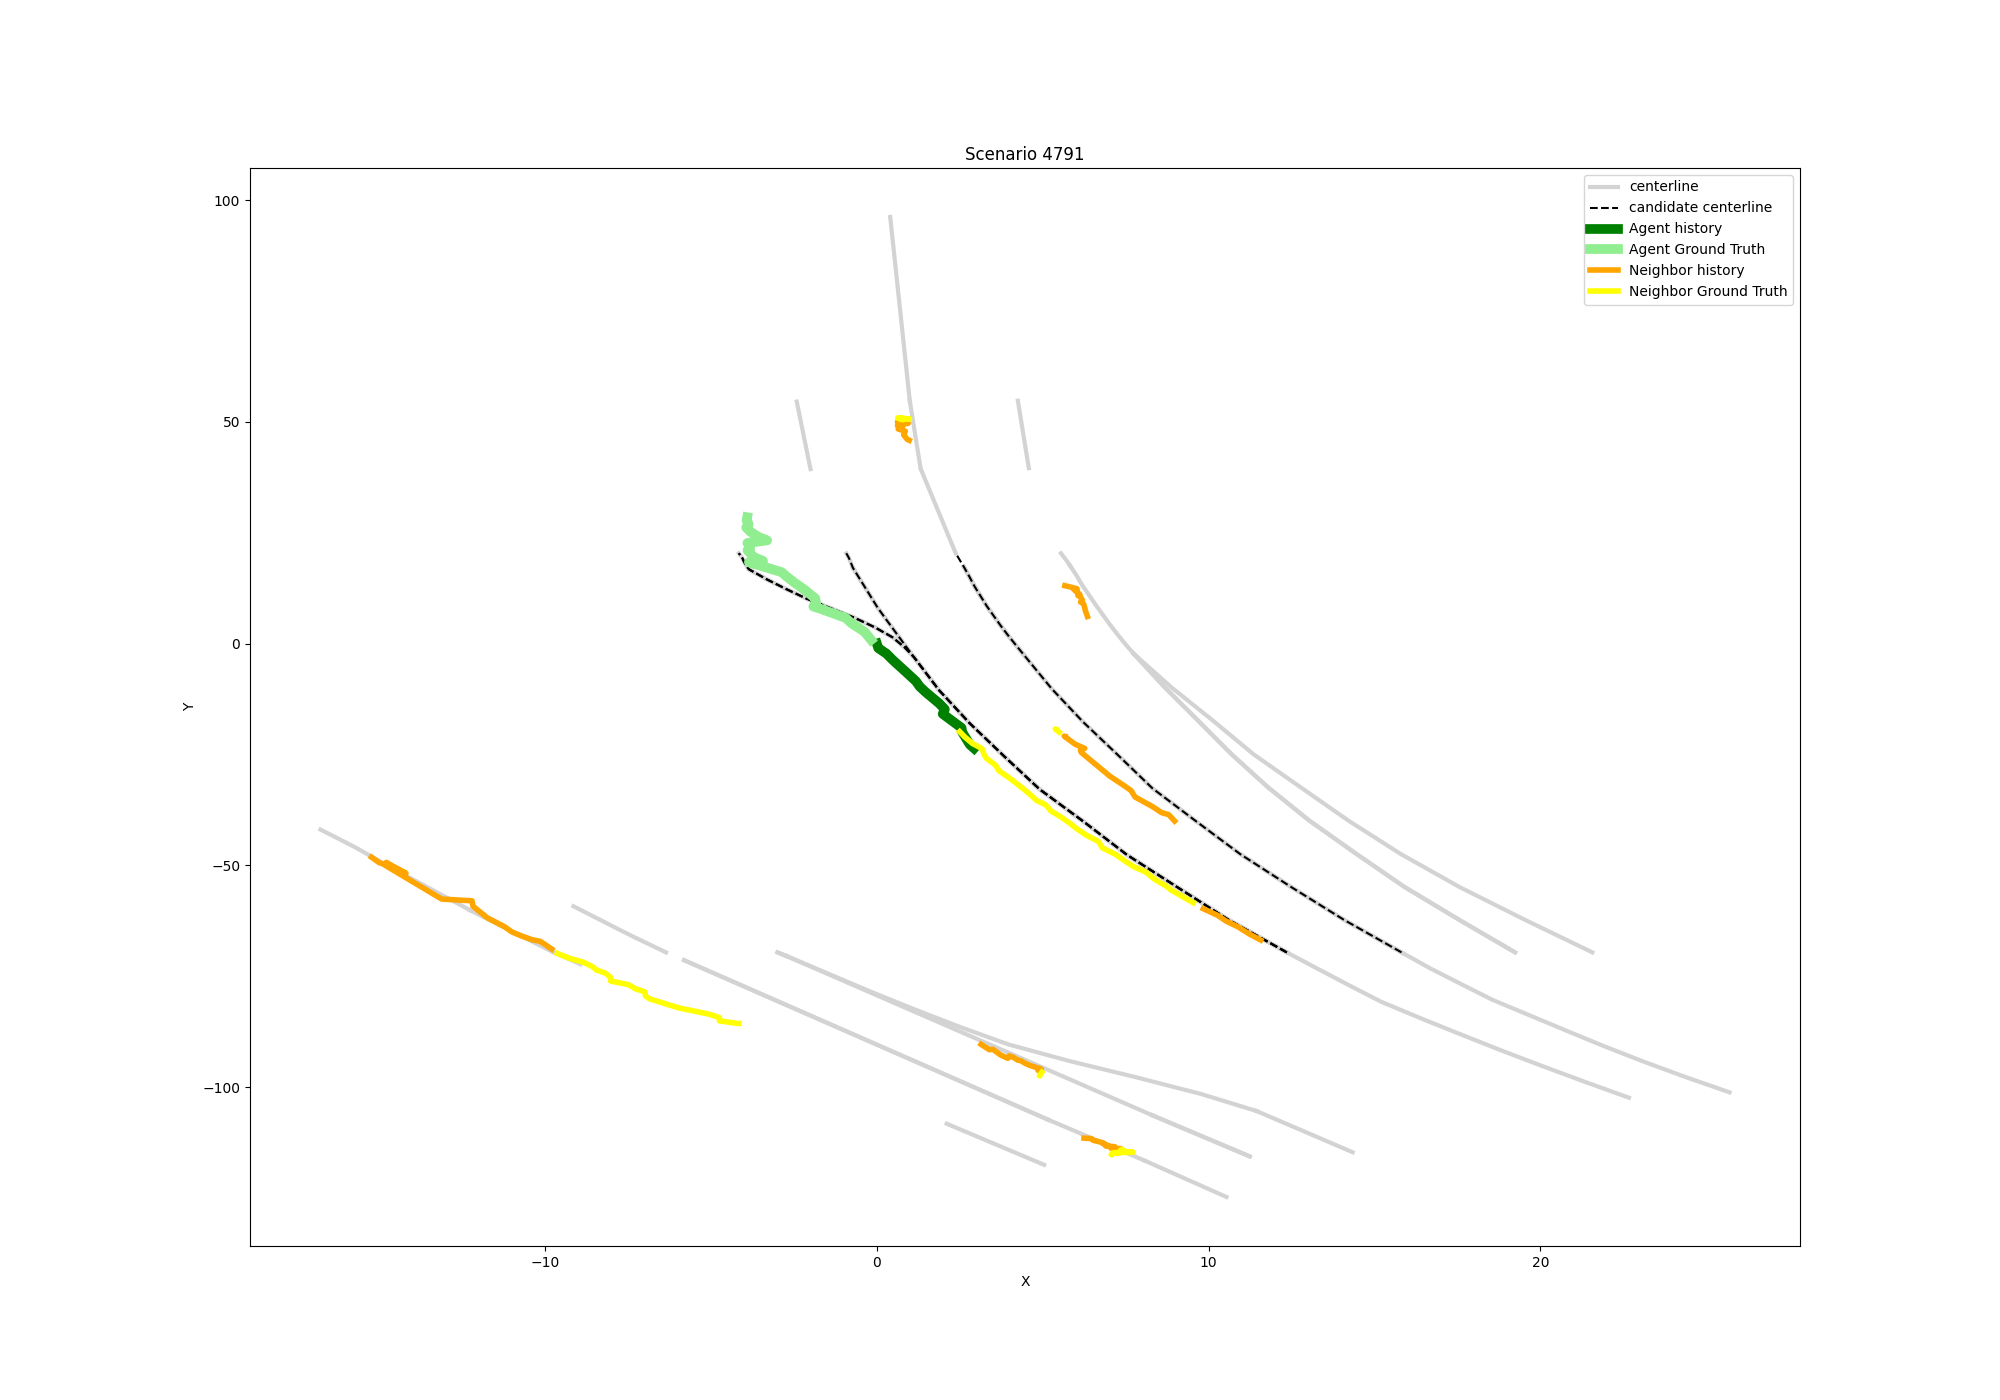
\includegraphics[width=0.9\textwidth]{images/scenario4791.png}
  \caption{Визуализација припремљених података - Пример 2}
  \label{scenario-example-4791}
\end{figure}

% ------------------------------------------------------------------------------

% ------------------------------------------------------------------------------
\chapter{Разрада}
\label{chp:razrada}
% ------------------------------------------------------------------------------

У изради...

% ------------------------------------------------------------------------------
\chapter{Закључак}
% ------------------------------------------------------------------------------
У изради...

% ------------------------------------------------------------------------------
% Literatura
% ------------------------------------------------------------------------------
\literatura

% ==============================================================================
% Završni deo teze i prilozi
\backmatter
% ==============================================================================

% ------------------------------------------------------------------------------
% Biografija kandidata
\begin{biografija}
\textbf{Момир Аџемовић} 
У изради...
\end{biografija}
% ------------------------------------------------------------------------------

\end{document} 